\documentclass[10pt,a4paper]{report}
\usepackage[utf8]{inputenc}
\usepackage{amsmath}
\usepackage{amsfonts}
\usepackage{amssymb}
\usepackage{graphicx,caption,subcaption}
\usepackage{varwidth,lipsum}

\usepackage{etoolbox}
\patchcmd{\thebibliography}{\chapter*}{\section*}{}{}

\author{Brendan Benshoof}
\title{Overview of Parallel Convex Hull Algorithms}
\begin{document}
\maketitle{}


\section{Introduction}

The Convex Hull problem can be considered one of the most well studied problems in computational geometry. There are numerous centralized algorithms and an achievable lower bound of O(nlog(n)) time (the sorting bound). It is surprising that there are a comparatively smaller number of parallel algorithms that have been researched.
Two major approaches (Divide and Conquer vs. Sampling) and three major algorithms (Atallah's algorithm\cite{Atallah1986Efficient}, qHull, and High Confidence sampling) dominate literature on the topic.
 

\subsection{Problem Formulation}

A convex hull, is a graph of a subset of a set of points in space such that the convex polytope described by that graph contains all points in the set.
In a geometric sense, this means describing a minimal space such that given any two points in a set, the line segment between them falls wholely within the set.

\begin{figure}[h!!]
        \centering
\begin{subfigure}[b]{0.4\textwidth}
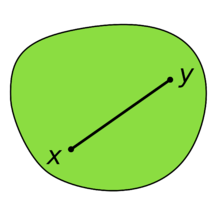
\includegraphics[width=\textwidth]{imgs/convex.png}

  \captionof{figure}{A convex set}

\end{subfigure}
\begin{subfigure}[b]{0.4\textwidth}
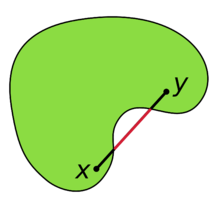
\includegraphics[width=\textwidth]{imgs/notconvex.png}
  \captionof{figure}{A non-convex (concave) set}

\end{subfigure}

\hspace*{15pt}\hbox{\scriptsize Credit:\thinspace{\small\itshape User A1 at en.wikipedia }}
\end{figure}

There are a variety of sequential algorithims to solve the 2d planar convex hull problem. Grahm's scan\cite{graham1972efficient} and QuickHull\cite{Barber1996} are worthy of note as solutions seeing common use. QuickHull is of specific interest as an examined line of parallel algorithims are based on it\cite{Stein2012CudaHull}\cite{SrikanthFast}.

The convex hull problem is involved in many common computations including collision detection and delunay-triangulation/voronoi tessellation.




\section{Overview of Literature}

Literature can be divided into two strong groupings. Those that derive from a high-probability of accuracy sampling method and those papers who's algorithm derives from divide and conquer approach.

The papers concerning divide and conquer approaches can be divided further into the papers that implement the parallel convex hull algorithm for EREW PRAM presented by Atallah et al versus the more modern algorithm which derive from the quick hull algorithm presented by Barber et al.


\section{Divide and Conquer methods}

Divide and Conquer is one of the basic computer science problem solving techniques. It's basis is in find a method to reduce a problem to simpler sub-problems then merge those sub-problems into a global solution. Breaking the global problem into sub-problems makes it well adapted to application in parallel algorithms, where each sub-problem can be solved in parallel, with most time being consumed by merging the sub-problems.


\subsection{Properties and applications}

Most papers discussed in this section derive from a divide and conquer method presented by Atallah et al\cite{Atallah1986Efficient}.
This algorithm is only defined for planar convex hull and does not extend readily into higher dimensions.


\subsection{Overview of literature}
Here I overview the papers I have categorized as Divide and Conquer approaches to parallel convex hull. They are presented in approximate order of development and publication. I present a summary of the contribution of the paper and a discussion of how it effected later work.


\subsubsection{Atallah et al}
Atallah et al\cite{Atallah1986Efficient} present a parallel variation of traditional divide and conquer algorithms for $O(n)$ processors. They present an $O(\log(n))$ time algorithm given $O(n)$ processors. Rather than splitting the problem space in an iterative binary fashion, they subdivide the problem space into $O(\sqrt{n})$ subdivisions. This allows the sub-problems each to be processed in parallel by $O(\sqrt{n})$ processors. This allows each sub-problem to be viewed independently as a problem with $O(n)$ input and $O(n)$ processors and this method can be applied recursively until trivial problems are established.

This elegant dividing of the problem space hinges on even subdivision of work. In the case of parallel convex hull, points are sorted along any convent axis using $O(\log(n))$ time (which dominates run-time).
Then $O(\sqrt{n})$ contiguous portions of $O(\sqrt{n})$ points are recursively solved and merged.

When recursively subdividing the space, while the ratio between bits of input and number of processors is $O(1)$ it is realistic to assume that data points outnumber the processors by more than three to one.
Thus, is subdivision reaches three or less points in a group, it can cease further subdivision as sets of points three or less have a trivial convex hull.
More realistically, once the subdivision cannot continue due to lack of processors, the convex hull of the $O(1)$ remaining points can be solved by a single processor in constant time using any one of the established sequential methods.
If all data has been provided initially to all nodes, the subdivision step can be preformed in $O(\log(n))$ time.


The bulk of computation is contained in the merging step. The recursive division step has created a merge tree, requiring $O(\log(n))$ iterations of the merging algorithm.
Once the points have been separated into trivial sub-problems they are merged in parallel in constant time. $O(\sqrt(n))$ subsets are merged using $O(n)$ processors, therefore we can assign one processor to each pair of potential merges.

%% How does merging actually happen in constant time per level

Atallah et al's algorithm is applied to more specific parallel computing architectures in later papers.



\subsubsection{Miller et al}

``Efficient parallel convex hull algorithms''\cite{Russ1988Efficient} was published in 1988, two years after Atallah et al's\cite{Atallah1986Efficient} foundational work.
Miller et al\cite{Russ1988Efficient} shows algorithms for preforming the convex hull operation given pre-sorted input on a variety of parallel architectures: a hypercube, pyramid,
tree, mesh-of-trees, mesh with reconfigurable bus, EREW PRAM, and a modified AKS network.
This paper allows the algorithim described by Atallah et al\cite{Atallah1986Efficient} to be applied to a variety of practical parallel computing architechtures while retaining the $O(log(n)$ time and $O(nlog(n)$ work properties. However becuase the algorithims are predicated on being pre-sorted (by order on any axis). This means that in cases of arbitrary input order, the algorithims are further bounded by the cost of sorting on that platform.


\subsubsection{Ferreira et al}

Ferreira et al\cite{Mohamadou1999Scalable} further extends Atallah et al onto a ``Coarse Grained'' computer model. This shows the algorithm can be preformed while preserving it's cost on a variety of limited communication systems. This genralization shows that further proof that runtime and work established by Atallah et al can be maintained on a given ``coarse grained'' parallel computer system.



\subsubsection{Amato et al}

In 1994 Amato et al published ``Parallel algorithms for higher - dimensional convex hulls''\cite{NancyParallel} which provides a EREW PRAM model for solving high dimension convex hulls using probabilistic linear programming methods in $O(log(n))$ time with $O(nlog(n)+n^{\frac{d}{2}})$ work.
Work in this paper is built on extensions of the parallel divide and conquer method into higher dimensions. (It is worth noting that this paper shares an author with Atallah et al in Michael Goodrich and it is clearly generalizing directly on his previous work.)

\subsection{QuickHull derived methods}

In practice, on GPU implementations, modern algorithms for convex hull calculation are based on the quick hull algorithm presented by Barber et al.

\begin{figure}[h!]
        \centering
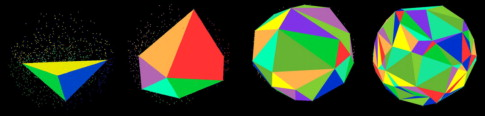
\includegraphics[width=\textwidth]{imgs/CUDAhull_example.jpg}

  \captionof{figure}{Visualization of QuickHull in 3D. This image is sourced from CUDAHull\cite{Stein2012CudaHull}}
\end{figure}

\subsubsection{Barber et al}
Barber et al\cite{Barber1996} does not present a parallel algorithm. It is included in this survey as it presents the QuickHull algorithm which other papers present a parallel variation of for GPU computing.

QuickHull's approach is to grow a area/volume which aggressively discards points and divides the remaining points into smaller sub-problems along the faces of the area's growth.
Barber et al presents QuickHull as a solution to 2d convex hull, however unlike many other sequential convex hull algorithms it is extended trivially into higher dimensions.
Like many other sequential convex hull algorithms, it requires $O(n\log(n))$ time (the sorting lower bound).

Quickhull can be formally described as follows:

Given $O(n)$ $d$-dimensional points in set $P$. 
Find $d+1$ maximal points and use them to form a d-dimensional simplex.
Discard all points in $P$ that are contained in this simplex.
Each face of the simplex partitions the remainder of $P$, recurse onto each of these partitions, utilizing the bounding face to bootstrap finding a new simplex.

It is important to note, that this algorithm only produces the set of points in the convex hull. In 2D, how these points are connected is trivial (sorted by angle around any point contained in the hull).
In higher dimensions, if a convex polytope is the desired output rather than a set of points, the partially correct linking information produced by the algorithm must be corrected to generate a correct convex polytope.
This cleanup operation is at worst $O(h)$ cost, where $h$ is the number of points on the convex hull.





\subsubsection{Srungarapu et al}

Srungarapu et al present ``Fast two dimensional convex hull on the GPU''\cite{SrikanthFast} in 2011, which describes an implementation of QuickHull in 2D for the CUDA platform.
It presents a $O(n\frac{log(n)}{p})$ time algorithm with $O(p)$ processors.
The point culling steps in QuickHull require minimal branching and is easily mapped to GPU parallel behavior. As the recursive are steps also similar, many recursions can be ran in parallel (each finding if a given point falls inside a given triangle).


\subsubsection{Stein et al}

Stein et al presented CudaHull\cite{Stein2012CudaHull} in 2012 which provides implementation of 3D QuickHull for CUDA. They provide a $O(\frac{n}{p}log(n))$ time algorithm, with a $O(h)$ sequential cleanup setup (where $h$ is the number of points on the convex hull) to provide a proper convex polytope description of the Hull (nontrivial in 3+ dimensions).
Their application is analogous to Srungarapu et al's\cite{SrikanthFast} with the added complexity of utilizing 3D tetrahedrons rather than 2D triangles. The inital cost is identical because the cost of testing if a point is contained in a simplex (of any dimension) is $O(d)$ which is assumed to be constant for these applications.
Because the final connections of points on the hull is not fully determined by QuickHull in higher dimensions, 



\section{Sampling Methods}


Sampling methods are generally not searching for solutions in a geometrically intuitive way.
They pose the convex hull problem as a linear programming problem and utilize conventional parallel search methods to generate a high confidence set of points as members of the convex hull.
This presents the problem, that while finding the set of points in a convex hull is a more computationally simple task than finding the entire hull, most applications require a full description of bother the verticies and edges of the convex hull polytope.
\subsection{Overview of literature}



\subsubsection{Dehne et al}
Dehne et al ``A Randomized Parallel 3D Convex Hull Algorithm for Coarse Grained Multicomputers''\cite{Dehne} supplies a high-probability of accuracy algorithm for 3d convex hull on EREW PRAM of O(log(n)) time by converting the convex hull problem into a linear program. The linear program solution only provides the set of points on the hull and a linear time method of building the polytope is utilized.

\subsubsection{Ghouse et al}

in 1997 Ghouse et al ``Fast randomized parallel methods for planar convex hull construction'' \cite{Mujtaba1997Fast} proposes the O(1) and O(nlog(n)) work algorithm for CRCW PRAM. The convex hull problem is presented as a linear programming problem and solved using probabilistic parallel linear programming techniques.
This work applies a previous published technique of ``in-place''\cite{ghouse1991place} algorithms operating on convex hulls.


It is worth noting that this work shares coauthor with Atallah et al in Michael Goodrich.



\section{Conclusions and Areas for New Research}

The field of works concerning Parallel Convex Hull algorithms is small but mature.
It will be difficult for new works to be published in this area simply because existing works have presented practical and provably optimal solutions to the Convex Hull problem.
Applications of these algorithms to solve practical problems and onto new computing platforms is the most clear space for future work.
Here I present some possible application areas and summaries of them.

\subsection{High performance convex hulls in higher-dimensional}
The Convex Hull problem provides solutions to many other geometric problems via embedding of those problems into a convex hull of higher dimension. There are not currently practical CUDA GPU tools for solving these higher dimensional convex hull problems.


\subsection{Parallel convex hulls to solve geometric problems in non-euclidean spaces}

Convex Hull algorithms in higher dimension provide solutions to delunay triangulation and other geometric problems in non-euclidean metric spaces. Such problems are seeing application in machine learning and network optimization. There are no current techniques for solving these problems on commodity parallel hardware.

\subsection{Parallelization of other Convex Hull Algorithms}
This servery only covers 3 sequential algorithms adapted for use in parallel computation. A wide field of sequential algorithms have not had published adaptations. 






\phantom{\cite{ChowParallel}}
\phantom{\cite{NancyParallel}}
\phantom{\cite{SrikanthFast}}
\phantom{\cite{Day1991Parallel}}

\phantom{\cite{reif1992optimal}}
\phantom{\cite{seidel1981convex}}









\bibliography{cites}
	\bibliographystyle{plain}

\end{document}